\documentclass[]{article}
\usepackage{lmodern}
\usepackage{amssymb,amsmath}
\usepackage{ifxetex,ifluatex}
\usepackage{fixltx2e} % provides \textsubscript
\ifnum 0\ifxetex 1\fi\ifluatex 1\fi=0 % if pdftex
  \usepackage[T1]{fontenc}
  \usepackage[utf8]{inputenc}
\else % if luatex or xelatex
  \ifxetex
    \usepackage{mathspec}
    \usepackage{xltxtra,xunicode}
  \else
    \usepackage{fontspec}
  \fi
  \defaultfontfeatures{Mapping=tex-text,Scale=MatchLowercase}
  \newcommand{\euro}{€}
\fi
% use upquote if available, for straight quotes in verbatim environments
\IfFileExists{upquote.sty}{\usepackage{upquote}}{}
% use microtype if available
\IfFileExists{microtype.sty}{%
\usepackage{microtype}
\UseMicrotypeSet[protrusion]{basicmath} % disable protrusion for tt fonts
}{}
\usepackage[margin=1in]{geometry}
\usepackage{color}
\usepackage{fancyvrb}
\newcommand{\VerbBar}{|}
\newcommand{\VERB}{\Verb[commandchars=\\\{\}]}
\DefineVerbatimEnvironment{Highlighting}{Verbatim}{commandchars=\\\{\}}
% Add ',fontsize=\small' for more characters per line
\usepackage{framed}
\definecolor{shadecolor}{RGB}{248,248,248}
\newenvironment{Shaded}{\begin{snugshade}}{\end{snugshade}}
\newcommand{\KeywordTok}[1]{\textcolor[rgb]{0.13,0.29,0.53}{\textbf{{#1}}}}
\newcommand{\DataTypeTok}[1]{\textcolor[rgb]{0.13,0.29,0.53}{{#1}}}
\newcommand{\DecValTok}[1]{\textcolor[rgb]{0.00,0.00,0.81}{{#1}}}
\newcommand{\BaseNTok}[1]{\textcolor[rgb]{0.00,0.00,0.81}{{#1}}}
\newcommand{\FloatTok}[1]{\textcolor[rgb]{0.00,0.00,0.81}{{#1}}}
\newcommand{\CharTok}[1]{\textcolor[rgb]{0.31,0.60,0.02}{{#1}}}
\newcommand{\StringTok}[1]{\textcolor[rgb]{0.31,0.60,0.02}{{#1}}}
\newcommand{\CommentTok}[1]{\textcolor[rgb]{0.56,0.35,0.01}{\textit{{#1}}}}
\newcommand{\OtherTok}[1]{\textcolor[rgb]{0.56,0.35,0.01}{{#1}}}
\newcommand{\AlertTok}[1]{\textcolor[rgb]{0.94,0.16,0.16}{{#1}}}
\newcommand{\FunctionTok}[1]{\textcolor[rgb]{0.00,0.00,0.00}{{#1}}}
\newcommand{\RegionMarkerTok}[1]{{#1}}
\newcommand{\ErrorTok}[1]{\textbf{{#1}}}
\newcommand{\NormalTok}[1]{{#1}}
\usepackage{longtable,booktabs}
\usepackage{graphicx}
\makeatletter
\def\maxwidth{\ifdim\Gin@nat@width>\linewidth\linewidth\else\Gin@nat@width\fi}
\def\maxheight{\ifdim\Gin@nat@height>\textheight\textheight\else\Gin@nat@height\fi}
\makeatother
% Scale images if necessary, so that they will not overflow the page
% margins by default, and it is still possible to overwrite the defaults
% using explicit options in \includegraphics[width, height, ...]{}
\setkeys{Gin}{width=\maxwidth,height=\maxheight,keepaspectratio}
\ifxetex
  \usepackage[setpagesize=false, % page size defined by xetex
              unicode=false, % unicode breaks when used with xetex
              xetex]{hyperref}
\else
  \usepackage[unicode=true]{hyperref}
\fi
\hypersetup{breaklinks=true,
            bookmarks=true,
            pdfauthor={Andrea Fernández, Liliana Millán},
            pdftitle={Proyecto Final: Multivariada},
            colorlinks=true,
            citecolor=blue,
            urlcolor=blue,
            linkcolor=magenta,
            pdfborder={0 0 0}}
\urlstyle{same}  % don't use monospace font for urls
\setlength{\parindent}{0pt}
\setlength{\parskip}{6pt plus 2pt minus 1pt}
\setlength{\emergencystretch}{3em}  % prevent overfull lines
\setcounter{secnumdepth}{5}

%%% Use protect on footnotes to avoid problems with footnotes in titles
\let\rmarkdownfootnote\footnote%
\def\footnote{\protect\rmarkdownfootnote}

%%% Change title format to be more compact
\usepackage{titling}
\setlength{\droptitle}{-2em}
  \title{Proyecto Final: Multivariada}
  \pretitle{\vspace{\droptitle}\centering\huge}
  \posttitle{\par}
  \author{Andrea Fernández, Liliana Millán}
  \preauthor{\centering\large\emph}
  \postauthor{\par}
  \predate{\centering\large\emph}
  \postdate{\par}
  \date{27/05/2015}


\usepackage{float}
\usepackage{morefloats}
\usepackage[spanish]{babel}
\usepackage{graphicx}
\usepackage{tcolorbox}
\usepackage{rotating}
\usepackage{longtable}
\usepackage{colortbl}

%\usepackage{natbib}
%\newenvironment{scaleb}{ \scalebox{0.4}{} {} }
%\newenvironment{scaleb}{ \tiny{} }
% biber
\usepackage[autostyle]{csquotes}

\usepackage[
    backend=biber,
    style=authoryear-icomp,
    sortlocale=de_DE,
    natbib=true,
    url=false,
    doi=true,
    eprint=false
]{biblatex}
\addbibresource{bibliografia.bib}

\usepackage[]{hyperref}
\hypersetup{
% Turn on this if you prefer to have links colored instead of marked with squares
colorlinks = true,
linkcolor = black,
urlcolor = blue,
citecolor = black,
% pdfpagemode = UseNone
}

\renewcommand\figurename{Figura}
\renewcommand\tablename{Tabla}

\newenvironment{myexampleblock}[1]{%
    \tcolorbox[beamer,%
    noparskip,breakable,
    colback=LightGreen,colframe=DarkGreen,%
    colbacklower=LimeGreen!75!LightGreen,%
    title=#1]}%
    {\endtcolorbox}

\newenvironment{myalertblock}[1]{%
    \tcolorbox[beamer,%
    noparskip,breakable,
    colback=LightCoral,colframe=DarkRed,%
    colbacklower=Tomato!75!LightCoral,%
    title=#1]}%
    {\endtcolorbox}

\newenvironment{myblock}[1]{%
    \tcolorbox[beamer,%
    noparskip,breakable,
    colback=LightBlue,colframe=DarkBlue,%
    colbacklower=DarkBlue!75!LightBlue,%
    title=#1]}%
    {\endtcolorbox}


\begin{document}

\maketitle


{
\hypersetup{linkcolor=black}
\setcounter{tocdepth}{2}
\tableofcontents
}
\pagebreak

\section{Modelo de Markov de estados
ocultos}\label{modelo-de-markov-de-estados-ocultos}

\subsection{Introducción}\label{introduccion}

Los modelos de HMM son modelos estadísticos que se utilizan en procesos
que se suponen Markovianos donde los estados no son visibles
directamente ---son latentes--- pero las variables influidas por estos
estados si lo son. El objetivo consiste en identificar estos estados
ocultos para conocer los estados, las transiciones entre los estados y
las probabilidades de cada estado sobre las variables a las que
influyen.

Los HMM han sido ampliamente utilizados en problemas de Procesamiento de
Lenguaje Natural (NLP) sobre todo para el reconocimiento del habla (Part
Of Speech, POS), etiquetado gramatical, reconocimiento de escritura
manual, etc. Stamp (2012)

\subsection{Objetivo}\label{objetivo}

Identificación de vocales y consonantes de un texto en español a través
de un modelo de HMM estimando sus parámetros.

\subsection{Especificación del modelo}\label{especificacion-del-modelo}

\begin{itemize}
\itemsep1pt\parskip0pt\parsep0pt
\item
  Utilizamos HMM con el algoritmo Baum-Welch para estimar los
  parámetros:
\end{itemize}

\begin{enumerate}
\def\labelenumi{\arabic{enumi}.}
\itemsep1pt\parskip0pt\parsep0pt
\item
  las probabilidades inciales de los estados
\item
  las probabilidades de transición entre estados
\item
  las probabilidades de cada símbolo de pertenecer a uno de los estados
\end{enumerate}

\begin{figure}[htbp]
\centering
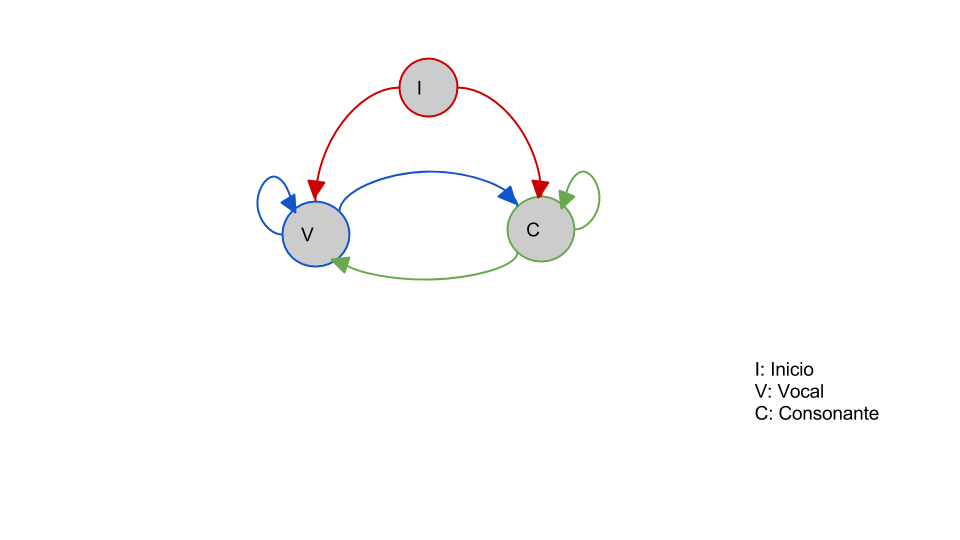
\includegraphics{modelo_vocales.png}
\caption{Diagrama de estados ocultos.}
\end{figure}

\subsubsection{Algoritmo Baum-Welch}\label{algoritmo-baum-welch}

\begin{itemize}
\itemsep1pt\parskip0pt\parsep0pt
\item
  Este algoritmo es una variante del EM visto en clase Frazzoli (2010);
  Bilmes (1998) . Iniciamos con un modelo sin `conocimiento'
\end{itemize}

$\pi$ = probabilidades de iniciar en cada estado

T= matriz de transición de estados

M= matriz de emisiones

$\lambda=(T,M,\pi)$

\begin{itemize}
\itemsep1pt\parskip0pt\parsep0pt
\item
  En cada iteración los valores de $\pi$, A y B se van actualizando
  hasta convergencia implementando el algoritmo forward-backward.
\end{itemize}

Definimos $\gamma_{k}(s)=Pr[X_{k}= s|Z,\lambda]$, la probabilidad de que
el sistema se encuentre en el estado $s$ en el $k$-ésimo tiempo, dada la
secuencia de observaciones $Z$ en el modelo $\lambda$ (forward-process).

\[
\gamma_{k}(s)=\frac{\alpha_{k}(s)\beta_{k}(s)}{Pr[Z|\lambda]}=\alpha_{k}(s)\beta_{k}(s){\sum_{s\epsilon\chi}\alpha_{t}(s)}
\]

Definimos $\xi_{k}(q,s)=Pr[X_{k}=q,X_{k+1}=s|Z,\lambda]$, la
probabilidad de estar en el estado $q$ al tiempo $k$ y en el estado $s$
en el tiempo $k+1$ dada la secuencia de observaciones en el modelo
actual de HMM (backward-process).

\[
\xi_{k}(q,s)=\eta_{k}\alpha_{k}(q)T_{q,s}M_{s,z_{k+1}}\beta_{k+1}(s)
\]

donde $\eta_{k}$ es un factor de normalización tal que
$\sum_{q,s}\xi_{k}(q,s)=1$.

Calculando $\gamma_{k}(s)$ y $\xi_{k}(q,s)$ podemos actualizar el modelo
$\lambda'=(T',M',\pi')$

\[
\pi'_{s}=\gamma_{1}(s)
\]

\[
T'_{q,s}=\frac{E[\#\phantom{a}de\phantom{a}transiciones\phantom{a}del\phantom{a}estado\phantom{a}q \phantom{a}al\phantom{a}s]}{E[\#\phantom{a}de\phantom{a}transiciones\phantom{a}del\phantom{a}estado\phantom{a}q]}=\frac{\sum_{k=1}^{t-1}\xi_{k(q,s)}}{\sum_{k=1}^{t-1}\gamma_{k}(q)}
\]

\[
M'_{s,m}=\frac{E[\#\phantom{a}de\phantom{a}veces\phantom{a}en\phantom{a}el\phantom{a}estado\phantom{a}s\phantom{a}cuando\phantom{a}la\phantom{a}observacion\phantom{a}fue\phantom{a}m]}{E[\# de veces en el estado s]}=\frac{\sum_{k=1}{t}\gamma_{k}(s)1(z_{k}=m)}{\sum_{k=1}^{t}\gamma_{k}(s)}
\]

\subsubsection{Suposiciones iniciales del
modelo}\label{suposiciones-iniciales-del-modelo}

\begin{itemize}
\itemsep1pt\parskip0pt\parsep0pt
\item
  Nuestra base será suponer que existen 2 estados: \textbf{Consonante} y
  \textbf{Vocal}\\
\item
  No conocemos con qué probabilidad de inicio estamos en Constante o en
  Vocal
\item
  No conocemos las probabilidades de transición entre estados
\item
  No conocemos las probabilidades de que cada símbolo del lenguaje
  pertenezca a uno de los estados
\end{itemize}

\subsection{Datos}\label{datos}

Intentamos ocupar los últimos 100 contenidos publicados en Quién.com y
CNNExpansión.com sin embargo sus corpus requieren de mucho de
preprocesamiento para eliminar encoding y caracteres extraños.

Decidimos tomar un corpus en español de un ejercicio realizado en
Métodos Analíticos correspondiente a un periodico español con 309,918
noticias

\subsubsection{Limpieza de Datos}\label{limpieza-de-datos}

\begin{itemize}
\itemsep1pt\parskip0pt\parsep0pt
\item
  Eliminamos signos de puntuación
\item
  Eliminamos dígitos
\item
  Eliminamos tabulaciones
\item
  Cambiamos todo el corpus a minúsculas
\item
  Dividimos cada palabra en sus letras respetando los espacios
\end{itemize}

\subsection{Metodología}\label{metodologia}

\begin{enumerate}
\def\labelenumi{\arabic{enumi}.}
\itemsep1pt\parskip0pt\parsep0pt
\item
  Limpieza de datos
\item
  Separar cada palabra en sus respectivas letras respetando espacios
\item
  Establecemos nuestro conocimiento a priori sobre las probabilidades
  iniciales de estados inicializando $\pi$. Dado que no conocemos mucho
  del proceso las establecemos muy cercanas a 0.5 (suman a 1)
\item
  Establecemos nuestro conocimiento a priori sobre las probabilidades de
  transición entre estados inicializando A. Dado que no conocemos mucho
  del proceso las establecemos cercanas a 0.5 pero agregando que creemos
  que es más probable la transición de vocal a consonante que de vocal a
  vocal, al igual que de consonante a vocal de que de consontante a
  consonante.
\item
  Establecemos nuestro conocimiento a priori sobre las probabilidades de
  cada símbolo a cada uno de los estados propuestos inicializando B.
  Dado que no conocemos mucho del proceso las establecemos dividiendo 1
  entre el número de símbolos posibles en el set de datos.
\item
  Inicialización de la HMM con los parámetros establecidos en el paso
  4,5 y 6.
\item
  Correr el algoritmo de Baum-Welch
\end{enumerate}

\subsection{Paquetes utlizadas}\label{paquetes-utlizadas}

\begin{itemize}
\item
  Paquete HMM de R Himmelmann (2010)
\item
  Algoritmo de Baum-Welch para estimación de parámetros de una HMM
\end{itemize}

\subsection{Resultados Español}\label{resultados-espanol}

Inicial sin conocimiento:

\begin{longtable}[c]{@{}ccc@{}}
\toprule\addlinespace
& V & C
\\\addlinespace
\midrule\endhead
& 0.5337 & 0.4662
\\\addlinespace
\bottomrule
\end{longtable}

Inicial después de Baum-Welch

\begin{longtable}[c]{@{}ccc@{}}
\toprule\addlinespace
& V & C
\\\addlinespace
\midrule\endhead
& 0.5337 & 0.4662
\\\addlinespace
\bottomrule
\end{longtable}

Transiciones sin conocimiento

\begin{longtable}[c]{@{}ccc@{}}
\toprule\addlinespace
& V & C
\\\addlinespace
\midrule\endhead
V & 0.3099 & 0.6900
\\\addlinespace
C & 0.5200 & 0.4799
\\\addlinespace
\bottomrule
\end{longtable}

Transiciones después de Baum-Welch

\begin{longtable}[c]{@{}ccc@{}}
\toprule\addlinespace
& V & C
\\\addlinespace
\midrule\endhead
V & 0.3045 & 0.6954
\\\addlinespace
C & 0.993 & 0.006
\\\addlinespace
\bottomrule
\end{longtable}

A continuación se identifican que las probabilides en el estado \emph{v}
de los símbolos \emph{a, e, i, o, u, ú} son mayores que las
probabilidades de estos símbolos al estado \emph{c}. De igual forma, las
probabilidades en el estado \emph{c} para los símbolos que \textbf{no}
son \emph{a, e, i, o, u, ú} son mayores que las probabilidades de estos
símbolos al estado \emph{v}.

\begin{figure}[htbp]
\centering
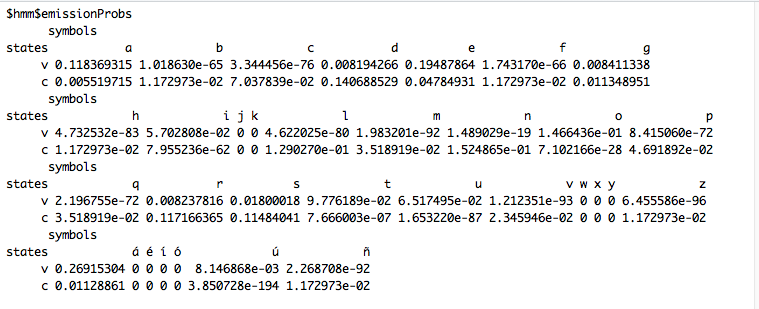
\includegraphics{salida_vocales.png}
\caption{Probabilidades de emisión del modelo en español.}
\end{figure}

\subsection{Resultados Griego}\label{resultados-griego}

Inicial sin conocimiento:

\begin{longtable}[c]{@{}ccc@{}}
\toprule\addlinespace
& V & C
\\\addlinespace
\midrule\endhead
& 0.53765 & 0.4234
\\\addlinespace
\bottomrule
\end{longtable}

Inicial después de Baum-Welch

\begin{longtable}[c]{@{}ccc@{}}
\toprule\addlinespace
& V & C
\\\addlinespace
\midrule\endhead
& 0.6117 & 0.3882
\\\addlinespace
\bottomrule
\end{longtable}

Transiciones sin conocimiento

\begin{longtable}[c]{@{}ccc@{}}
\toprule\addlinespace
& V & C
\\\addlinespace
\midrule\endhead
V & 0.3558 & 0.6441
\\\addlinespace
C & 0.5161 & 0.4838
\\\addlinespace
\bottomrule
\end{longtable}

Transiciones después de Baum-Welch

\begin{longtable}[c]{@{}ccc@{}}
\toprule\addlinespace
& V & C
\\\addlinespace
\midrule\endhead
V & 0.0093 & 0.9906
\\\addlinespace
C & 0.6178 & 0.3821
\\\addlinespace
\bottomrule
\end{longtable}

En griego las vocales corresponden a los símbolos:

\begin{longtable}[c]{@{}cc@{}}
\toprule\addlinespace
Griego & ~Vocal
\\\addlinespace
\midrule\endhead
A,$\alpha$ & a
\\\addlinespace
E,$\epsilon$ & e
\\\addlinespace
I,$\iota$ & i
\\\addlinespace
O,$\omicron$ & o
\\\addlinespace
Y,$\upsilon$ & u
\\\addlinespace
\bottomrule
\end{longtable}

A continuación se identifican que las probabilides en el estado \emph{v}
de los símbolos
$\alpha$,$\epsilon$,$\iota$,$\omicron$,$\upsilon$,$\epsilon$ acentuado,
son mayores que las probabilidades de estos símbolos al estado \emph{c}.
De igual forma, las probabilidades en el estado \emph{c} para los
símbolos que \textbf{no} son
$\alpha$,$\epsilon$,$\iota$,$\omicron$,$\upsilon$,$\epsilon$ acentuado
son mayores que las probabilidades de estos símbolos al estado \emph{v}.

\begin{figure}[htbp]
\centering
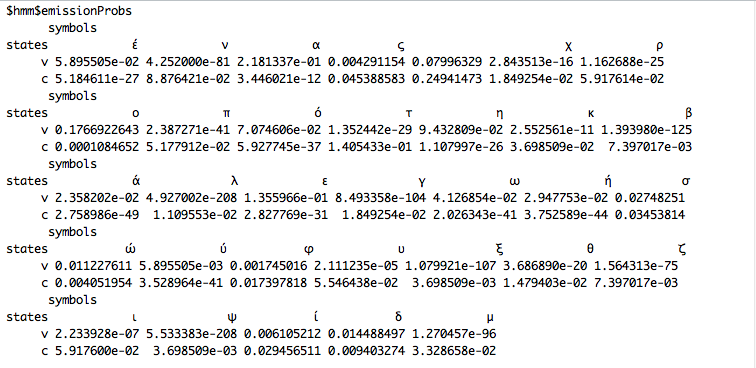
\includegraphics{salida_vocales_griego.png}
\caption{Probabilidades de emisión del modelo en griego.}
\end{figure}

\pagebreak

\subsection{Código}\label{codigo}

\subsubsection{Español}\label{espanol}

\begin{Shaded}
\begin{Highlighting}[]
\KeywordTok{library}\NormalTok{(HMM)}

\NormalTok{periodico <-}\StringTok{ }\KeywordTok{scan}\NormalTok{(}\DataTypeTok{file=}\StringTok{'./datos/Es_Newspapers.txt'}\NormalTok{, }\DataTypeTok{sep=}\StringTok{"}\CharTok{\textbackslash{}n}\StringTok{"}\NormalTok{, }
                  \DataTypeTok{what =} \KeywordTok{character}\NormalTok{())}

\CommentTok{#limpieza de datos}
\NormalTok{for(i in }\DecValTok{1}\NormalTok{:}\KeywordTok{length}\NormalTok{(periodico)) \{}
  \NormalTok{periodico[i] <-}\StringTok{ }\KeywordTok{gsub}\NormalTok{(}\StringTok{"[[:punct:]]"}\NormalTok{,}\StringTok{""}\NormalTok{,}\KeywordTok{unlist}\NormalTok{(periodico[i]))}
  \NormalTok{periodico[i] <-}\StringTok{ }\KeywordTok{gsub}\NormalTok{(}\StringTok{"[[:digit:]]"}\NormalTok{,}\StringTok{""}\NormalTok{,}\KeywordTok{unlist}\NormalTok{(periodico[i]))}
  \NormalTok{periodico[i] <-}\StringTok{ }\KeywordTok{tolower}\NormalTok{(periodico[i])}
  \NormalTok{periodico[i] <-}\StringTok{ }\KeywordTok{gsub}\NormalTok{(}\StringTok{"[[:space:]]"}\NormalTok{,}\StringTok{" "}\NormalTok{,}\KeywordTok{unlist}\NormalTok{(periodico[i]))}
\NormalTok{\}}


\CommentTok{#separando a letras}
\NormalTok{for (i in }\DecValTok{1}\NormalTok{) \{}
  \NormalTok{texto <-}\StringTok{ }\NormalTok{periodico[i]}
  \NormalTok{if(i ==}\StringTok{ }\DecValTok{1}\NormalTok{)\{}
    \NormalTok{obsv <-}\StringTok{ }\KeywordTok{as.data.frame}\NormalTok{(}\KeywordTok{unlist}\NormalTok{(}\KeywordTok{strsplit}\NormalTok{(texto, }\DataTypeTok{split=}\StringTok{""}\NormalTok{)), }
                          \DataTypeTok{stringsAsFactors=}\OtherTok{FALSE}\NormalTok{)}
  \NormalTok{\} else \{}
    \NormalTok{obsv <-}\StringTok{ }\KeywordTok{rbind}\NormalTok{(obsv, }\KeywordTok{as.data.frame}\NormalTok{(}\KeywordTok{unlist}\NormalTok{(}\KeywordTok{strsplit}\NormalTok{(texto, }\DataTypeTok{split=}\StringTok{""}\NormalTok{)), }
                                      \DataTypeTok{stringsAsFactors=}\OtherTok{FALSE}\NormalTok{))}
  \NormalTok{\}}
\NormalTok{\}}
\KeywordTok{names}\NormalTok{(obsv) <-}\StringTok{ "letter"}


\NormalTok{states =}\StringTok{ }\KeywordTok{c}\NormalTok{(}\StringTok{"v"}\NormalTok{,}\StringTok{"c"}\NormalTok{)}
\NormalTok{symbols =}\StringTok{ }\KeywordTok{c}\NormalTok{(}\StringTok{"a"}\NormalTok{,}\StringTok{"b"}\NormalTok{,}\StringTok{"c"}\NormalTok{,}\StringTok{"d"}\NormalTok{,}\StringTok{"e"}\NormalTok{,}\StringTok{"f"}\NormalTok{,}\StringTok{"g"}\NormalTok{,}\StringTok{"h"}\NormalTok{,}\StringTok{"i"}\NormalTok{,}\StringTok{"j"}\NormalTok{,}\StringTok{"k"}\NormalTok{,}\StringTok{"l"}\NormalTok{,}\StringTok{"m"}\NormalTok{,}\StringTok{"n"}\NormalTok{,}\StringTok{"o"}\NormalTok{,}\StringTok{"p"}\NormalTok{,}\StringTok{"q"}\NormalTok{,}
            \StringTok{"r"}\NormalTok{,}\StringTok{"s"}\NormalTok{,}\StringTok{"t"}\NormalTok{,}\StringTok{"u"}\NormalTok{,}\StringTok{"v"}\NormalTok{,}\StringTok{"w"}\NormalTok{,}\StringTok{"x"}\NormalTok{,}\StringTok{"y"}\NormalTok{,}\StringTok{"z"}\NormalTok{,}\StringTok{" "}\NormalTok{,}\StringTok{"á"}\NormalTok{,}\StringTok{"é"}\NormalTok{,}\StringTok{"í"}\NormalTok{,}\StringTok{"ó"}\NormalTok{,}\StringTok{"ú"}\NormalTok{,}\StringTok{"ñ"}\NormalTok{)}
\CommentTok{#probabilidades iniciales de lso estados}
\NormalTok{random_num <-}\StringTok{ }\KeywordTok{runif}\NormalTok{(}\DecValTok{1}\NormalTok{,}\FloatTok{0.5}\NormalTok{,}\FloatTok{0.7}\NormalTok{)}
\NormalTok{startProbs =}\StringTok{ }\KeywordTok{matrix}\NormalTok{(}\KeywordTok{c}\NormalTok{(random_num, }\DecValTok{1}\NormalTok{-random_num), }\DecValTok{2}\NormalTok{)}

\NormalTok{random_num <-}\StringTok{ }\KeywordTok{runif}\NormalTok{(}\DecValTok{1}\NormalTok{, }\FloatTok{0.5}\NormalTok{,}\FloatTok{0.7}\NormalTok{)}
\NormalTok{random_num_2 <-}\StringTok{ }\KeywordTok{runif}\NormalTok{(}\DecValTok{1}\NormalTok{, }\FloatTok{0.5}\NormalTok{,}\FloatTok{0.7}\NormalTok{)}
\NormalTok{transProbs <-}\StringTok{ }\KeywordTok{matrix}\NormalTok{(}\KeywordTok{c}\NormalTok{(}\DecValTok{1}\NormalTok{-random_num, random_num_2, }
                       \NormalTok{random_num, }\DecValTok{1}\NormalTok{-random_num_2), }\DecValTok{2}\NormalTok{)}
  
\NormalTok{random_nums <-}\StringTok{ }\KeywordTok{data.frame}\NormalTok{(}\KeywordTok{runif}\NormalTok{(}\DecValTok{33}\NormalTok{,}\FloatTok{0.030}\NormalTok{,}\FloatTok{0.034}\NormalTok{), }\KeywordTok{runif}\NormalTok{(}\DecValTok{33}\NormalTok{,}\FloatTok{0.030}\NormalTok{,}\FloatTok{0.034}\NormalTok{))}
\NormalTok{random_nums <-}\StringTok{ }\KeywordTok{data.frame}\NormalTok{(}\KeywordTok{rep}\NormalTok{(}\DecValTok{1}\NormalTok{/}\DecValTok{33}\NormalTok{,}\DecValTok{33}\NormalTok{), }\KeywordTok{rep}\NormalTok{(}\DecValTok{1}\NormalTok{/}\DecValTok{33}\NormalTok{,}\DecValTok{33}\NormalTok{))}
\NormalTok{emissionProbs=}\KeywordTok{as.matrix}\NormalTok{(random_nums)}
\NormalTok{inithmm <-}\StringTok{ }\KeywordTok{initHMM}\NormalTok{(states, symbols, }\DataTypeTok{startProbs=}\NormalTok{startProbs, }
                   \DataTypeTok{transProbs=}\NormalTok{transProbs, }
                   \DataTypeTok{emissionProbs=}\NormalTok{emissionProbs)}
\NormalTok{bw <-}\StringTok{ }\KeywordTok{baumWelch}\NormalTok{(inithmm, obsv$letter)}
\NormalTok{bw}
\end{Highlighting}
\end{Shaded}

\subsubsection{Griego}\label{griego}

\begin{Shaded}
\begin{Highlighting}[]
\KeywordTok{library}\NormalTok{(HMM)}

\KeywordTok{setwd}\NormalTok{(}\StringTok{"/Users/Lili/Documents/itam/estadistica_multivariada_y_datos_categoricos/}
\StringTok{      examenes/final"}\NormalTok{)}


\NormalTok{periodico <-}\StringTok{ }\KeywordTok{scan}\NormalTok{(}\DataTypeTok{file=}\StringTok{'griego_test.txt'}\NormalTok{, }\DataTypeTok{sep=}\StringTok{"}\CharTok{\textbackslash{}n}\StringTok{"}\NormalTok{, }\DataTypeTok{what =} \KeywordTok{character}\NormalTok{())}



\NormalTok{for(i in }\DecValTok{1}\NormalTok{:}\KeywordTok{length}\NormalTok{(periodico)) \{}
  \NormalTok{periodico[i] <-}\StringTok{ }\KeywordTok{gsub}\NormalTok{(}\StringTok{"[[:punct:]]"}\NormalTok{,}\StringTok{""}\NormalTok{,}\KeywordTok{unlist}\NormalTok{(periodico[i]))}
  \NormalTok{periodico[i] <-}\StringTok{ }\KeywordTok{gsub}\NormalTok{(}\StringTok{"[[:digit:]]"}\NormalTok{,}\StringTok{""}\NormalTok{,}\KeywordTok{unlist}\NormalTok{(periodico[i]))}
  \NormalTok{periodico[i] <-}\StringTok{ }\KeywordTok{tolower}\NormalTok{(periodico[i])}
  \NormalTok{periodico[i] <-}\StringTok{ }\KeywordTok{gsub}\NormalTok{(}\StringTok{"[[:space:]]"}\NormalTok{,}\StringTok{" "}\NormalTok{,}\KeywordTok{unlist}\NormalTok{(periodico[i]))}
\NormalTok{\}}



\NormalTok{for (i in }\DecValTok{1}\NormalTok{) \{}
  \NormalTok{texto <-}\StringTok{ }\NormalTok{periodico[i]}
  \NormalTok{if(i ==}\StringTok{ }\DecValTok{1}\NormalTok{)\{}
    \NormalTok{obsv <-}\StringTok{ }\KeywordTok{as.data.frame}\NormalTok{(}\KeywordTok{unlist}\NormalTok{(}\KeywordTok{strsplit}\NormalTok{(texto, }\DataTypeTok{split=}\StringTok{""}\NormalTok{)), }
                          \DataTypeTok{stringsAsFactors=}\OtherTok{FALSE}\NormalTok{)}
  \NormalTok{\} else \{}
    \NormalTok{obsv <-}\StringTok{ }\KeywordTok{rbind}\NormalTok{(obsv, }\KeywordTok{as.data.frame}\NormalTok{(}\KeywordTok{unlist}\NormalTok{(}\KeywordTok{strsplit}\NormalTok{(texto, }\DataTypeTok{split=}\StringTok{""}\NormalTok{)), }
                                      \DataTypeTok{stringsAsFactors=}\OtherTok{FALSE}\NormalTok{))}
  \NormalTok{\}}
\NormalTok{\}}
\KeywordTok{names}\NormalTok{(obsv) <-}\StringTok{ "letter"}

\CommentTok{#obsv <- obsv[-which(obsv$letter=="¾"),]}
\CommentTok{#obsv <- obsv[-which(obsv == "å")]}

\NormalTok{states =}\StringTok{ }\KeywordTok{c}\NormalTok{(}\StringTok{"v"}\NormalTok{,}\StringTok{"c"}\NormalTok{)}
\NormalTok{symbols =}\StringTok{ }\KeywordTok{c}\NormalTok{(}\StringTok{"έ"}\NormalTok{,}\StringTok{"ν"}\NormalTok{,}\StringTok{"α"}\NormalTok{,}\StringTok{"ς"}\NormalTok{,}\StringTok{" "}\NormalTok{,}\StringTok{"χ"}\NormalTok{,}\StringTok{"ρ"}\NormalTok{,}\StringTok{"ο"}\NormalTok{,}\StringTok{"π"}\NormalTok{,}\StringTok{"ό"}\NormalTok{,}\StringTok{"τ"}\NormalTok{,}\StringTok{"η"}\NormalTok{,}\StringTok{"κ"}\NormalTok{,}\StringTok{"β"}\NormalTok{,}\StringTok{"ά"}\NormalTok{,}
            \StringTok{"λ"}\NormalTok{,}\StringTok{"ε"}\NormalTok{,}\StringTok{"γ"}\NormalTok{,}\StringTok{"ω"}\NormalTok{,}\StringTok{"ή"}\NormalTok{,}\StringTok{"σ"}\NormalTok{,}\StringTok{"ώ"}\NormalTok{,}\StringTok{"ύ"}\NormalTok{,}\StringTok{"φ"}\NormalTok{,}\StringTok{"υ"}
            \NormalTok{,}\StringTok{"ξ"}\NormalTok{,}\StringTok{"θ"}\NormalTok{,}\StringTok{"ζ"}\NormalTok{,}\StringTok{"ι"}\NormalTok{,}\StringTok{"ψ"}\NormalTok{,}\StringTok{"ί"}\NormalTok{,}\StringTok{"δ"}\NormalTok{,}\StringTok{"μ"}\NormalTok{)}
\CommentTok{#probabilidades iniciales de lso estados}
\NormalTok{random_num <-}\StringTok{ }\KeywordTok{runif}\NormalTok{(}\DecValTok{1}\NormalTok{,}\FloatTok{0.5}\NormalTok{,}\FloatTok{0.7}\NormalTok{)}
\NormalTok{startProbs =}\StringTok{ }\KeywordTok{matrix}\NormalTok{(}\KeywordTok{c}\NormalTok{(random_num, }\DecValTok{1}\NormalTok{-random_num), }\DecValTok{2}\NormalTok{)}

\NormalTok{random_num <-}\StringTok{ }\KeywordTok{runif}\NormalTok{(}\DecValTok{1}\NormalTok{, }\FloatTok{0.5}\NormalTok{,}\FloatTok{0.7}\NormalTok{)}
\NormalTok{random_num_2 <-}\StringTok{ }\KeywordTok{runif}\NormalTok{(}\DecValTok{1}\NormalTok{, }\FloatTok{0.5}\NormalTok{,}\FloatTok{0.7}\NormalTok{)}
\NormalTok{transProbs <-}\StringTok{ }\KeywordTok{matrix}\NormalTok{(}\KeywordTok{c}\NormalTok{(}\DecValTok{1}\NormalTok{-random_num,random_num_2,  }
                       \NormalTok{random_num,}\DecValTok{1}\NormalTok{-random_num_2), }\DecValTok{2}\NormalTok{)}
  
\CommentTok{#random_nums <- data.frame(runif(31,0.030,0.034), runif(33,0.030,0.034))}
\NormalTok{random_nums <-}\StringTok{ }\KeywordTok{data.frame}\NormalTok{(}\KeywordTok{rep}\NormalTok{(}\DecValTok{1}\NormalTok{/}\KeywordTok{length}\NormalTok{(symbols),}\KeywordTok{length}\NormalTok{(symbols)), }
                          \KeywordTok{rep}\NormalTok{(}\DecValTok{1}\NormalTok{/}\KeywordTok{length}\NormalTok{(symbols),}\KeywordTok{length}\NormalTok{(symbols)))}
\NormalTok{emissionProbs=}\KeywordTok{as.matrix}\NormalTok{(random_nums)}
\NormalTok{inithmm <-}\StringTok{ }\KeywordTok{initHMM}\NormalTok{(states, symbols, }\DataTypeTok{startProbs=}\NormalTok{startProbs, }
                   \DataTypeTok{transProbs=}\NormalTok{transProbs, }
                   \DataTypeTok{emissionProbs=}\NormalTok{emissionProbs)}
\NormalTok{bw <-}\StringTok{ }\KeywordTok{baumWelch}\NormalTok{(inithmm, obsv$letter)}
\NormalTok{bw}
\end{Highlighting}
\end{Shaded}

\pagebreak

\subsection{Bibliografía}\label{bibliografia}

{[}1{]} J. Bilmes. \emph{A Gentle Tutorial of the EM Algorithm and its
Application to Parameter Estimation for Gaussian Mixture and Hidden
Markov Models}. Tech. rep. International Computer Science Institute,
Berkeley, abr. 1998.

{[}2{]} E. Frazzoli. \emph{Principles of Autonomy and Decision Making}.
Tech. rep. Massachusetts Insitute of Techonolgy (MIT), nov. 2010.

{[}3{]} D. L. Himmelmann. \emph{HMM: Hidden Markov Models}. R package
version 1.0. 2010.

{[}4{]} M. Stamp. \emph{A Revealing Introduction to Hidden Markov
Models}. Tech. rep. San Jose State University, sep. 2012.

\pagebreak

\section{Regresión multinivel y
postestratificación}\label{regresion-multinivel-y-postestratificacion}

\subsection{Introducción}\label{introduccion-1}

Este documento detalla el método de regresión multinivel y
postestratificación (MRP por sus siglas en inglés) para poder corregir
sesgo de selección en los datos recolectados a través de una encuesta
con diseño muestral no probabilístico por cuotas, como las realizadas en
los diagnósticos participativos de Morelos de 2013 y 2014. El objetivo
es construir estimadores precisos sobre la población objetivo.

Existen varios factores que pueden afectar o no la calidad de los datos
recolectados en una encuesta. La recolección de encuestas realizadas en
Morelos en 2013 y 2014 se realizó con las siguientes características: a)
muestreo no probabilístico por cuotas con inferencia basada en modelos y
no en diseño, b) administración remota del proceso de la encuesta o
trabajo de campo, c) recolección de datos asistida por tabletas
móviles\footnote{En particular, la recolección de información de
  encuestas asistida por computadoras tiene la ventaja de que las
  respuestas son capturadas inmediatamente de las personas encuestadas y
  guardadas en una base de datos para su procesamiento futuro. Esto
  reduce tiempos, costos y errores de transcripción. Facilita, además,
  flujos complicados en las respuestas del cuestionario, filtros,
  control de la validez de las respuestas, inclusión de elementos
  multimedia, entre otros (Vehovar and Manfreda, 2008, p.~179). Así
  mismo, permite tener un mejor manejo del trabajo de campo pues se
  pueden ir examinando tanto el avance como los resultados de manera
  paralela al levantamiento.}.

Fricker (2008, p.~198) desglosa cuatro posibles fuentes de error en
encuestas:

\begin{enumerate}
\def\labelenumi{\arabic{enumi}.}
\item
  \textbf{Error de cobertura}: parte de la población no puede ser
  incluida en la muestra. Para reducir el error de cobertura, las
  técnicas usadas comúnmente son tres: a) especificar un marco de
  muestreo tan completo como sea posible, b) utilizar una estrategia de
  muestreo sin marco en donde casi toda la población tenga una
  probabilidad de ser elemento de la muestra, c) post-estratificación:
  ponderar la muestra para que sea equivalente a la población de
  inferencia en ciertas características.
\item
  \textbf{Error de muestreo}: los resultados de diferentes muestras
  serán distintos. En una encuesta con muestreo aleatorio, el error de
  muestreo decrece cuando se incrementa el tamaño de muestra\footnote{Nótese
    que esto es cierto debido a que, si la muestra es aleatoria,
    entonces el estimador tiende asintóticamente al verdadero valor del
    parámetro. Sin embargo, si no es aleatoria, no hay control en los
    sesgos y esta propiedad no está garantizada.}.
\item
  \textbf{Errores por no respuesta}: ocurren cuando no se recolectan los
  datos de una unidad muestral completa o de respuestas parciales. La
  tasa de no respuesta, la razón entre el número de encuestados y el
  tamaño de muestra, es una medida de cuán posible es generalizar los
  resultados de una encuesta pues hay menor sesgo de no respuesta.
\item
  \textbf{Errores de medición}: la respuesta de la encuesta difiere de
  la ``respuesta verdadera''. Por ejemplo, cuando el encuestado no
  responde honestamente, cuando se interpreta mal la pregunta o se
  cometen errores al contestar, al hacer la pregunta o al transcribirla.
\end{enumerate}

La estructura de este documento es la siguiente: en la sección dos se
especifican los tipos de muestreo y se profundiza sobre las ventajas y
desventajas que ofrecen las encuestas de diseño no probabilístico. Con
este tipo de datos, el problema más importante es el sesgo de selección
que puede tener una muestra. En la sección tres se enlistan varios
métodos que ayudan a corregir este error y en la sección cuatro se
profundiza en particular sobre la regresión multinivel y
postestratificación para este caso en particular. En la sección cinco se
muestra un ejemplo práctico del uso de este método para las encuestas de
Morelos de 2013 y 2014.

\subsection{Muestreo}\label{muestreo}

Una buena muestra es intuitivamente, aquella que es representativa de la
población de la que fue extraida, es decir, que los resultados de los
datos recolectados de ésta son consistentes con los resultados que
hubiésemos obtenido si se hubiera censado a la población (Fricker, 2008,
p.~197).

El muestreo de encuestas puede ser agrupado en dos categorías: muestreo
\emph{probabilístico} y \emph{no probabilístico}. De la definición de
muestreo probabilístico sabemos que cada individuo en la población tiene
una probabilidad positiva y conocida de ser seleccionado\footnote{Es
  precisamente esta propiedad lo que permite realizar inferencias acerca
  de la población basadas en diseño: la aleatorización en la selección
  permite tener una estimación puntual y de intervalo para los
  parámetros que se desean conocer.}. En el segundo grupo se incluye,
por ejemplo, el muestreo propositivo (Little, 2014, p.~415). En este
tipo de muestreos la probabilidad de inclusión de cada unidad no puede
determinarse o es decisión de los individuos el participar o no en la
encuesta (\emph{opt-in}).

Una de las formas más comunes de muestreo no probabilístico es el
muestreo por cuotas. Las unidades son elegidas tal que la muestra posea
la misma distribución que una característica conocida de la población.
Por ejemplo, si se conoce la distribución de edad y género en la
población, se elige una muestra equivalente a esta distribución. En este
ejemplo, los entrevistadores reciben una cuota por cada grupo de edad y
género y entrevistan a individuos hasta que la cuota se cumple.

El muestreo por cuotas es similar al muestreo estratificado pues agrupa
unidades similares. Sin embargo, difieren en la manera en la que las
unidades son seleccionadas. Cuando el muestreo es probabilístico, las
unidades de la muestra son seleccionadas de manera aleatoria mientras
que en muestreo por cuotas se le deja al entrevistador elegir a quién
muestrea. Esto resulta en sesgo de selección. Para hacer inferencias
acerca de la población a partir de una muestra extraida por cuotas no
probabilística es necesario suponer que las personas que fueron
seleccionadas son similares a las que no lo fueron. Este supuesto es
fuerte y raramente válido.

Pese a que, en general, muestras no probabilísticas no permiten que se
realicen afirmaciones sobre toda la población de inferencia, tienen
muchas ventajas que se enlistan a continuación:

\begin{itemize}
\itemsep1pt\parskip0pt\parsep0pt
\item
  Son relativamente más baratas.
\item
  Son más fáciles de administrar.
\item
  Tienen la característica deseable de satisfacer proporciones de la
  población.
\item
  Son más adecuadas para estudios cualitativos profundos cuyo objetivo
  es entender fenómenos sociales complejos, por ejemplo, véase Marshall
  (1996); Small (2009).
\item
  La literatura indica que son apropiadas si se está interesado
  solamente en los casos específicos estudiados.
\item
  La inferencia basada en diseño tiene la limitante de ser asintótica y
  tiene pocas herramientas para muestras pequeñas o áreas de estimación
  pequeñas. Para estos casos, el muestreo no probabilístico es una buena
  alternativa.
\item
  Son una alternativa cuando no existe un marco muestral\footnote{Éste
    es el caso del levantamiento en Morelos pues no se buscaba realizar
    una encuesta en viviendas (para la cuál si existe un marco muestral)
    sino de personas en el espacio público. No existe un listado que
    permita realizar una selección aleatoria, es decir, no hay marco
    muestral.}.
\end{itemize}

Algunas diferencias que es importante considerar entre muestreos
probabilísticos y no probabilísticos son los siguientes:

\begin{itemize}
\itemsep1pt\parskip0pt\parsep0pt
\item
  En muestreo probabilístico, cuando no hay un modelo para predecir los
  casos excluidos de la muestra (los errores antes mencionados 1. de
  cobertura y 3. por no respuesta), la verosimilitud calculada es
  básicamente no informativa. Esto los haría equivalentes en poder de
  inferencia a modelos no probabilísticos pero con el costo añadido del
  diseño y los costos de administración adicionales (Little, 2014,
  p.~422).
\item
  El gran problema de muestreos no probabilísticos basados en cuotas
  deriva de no conocer los sesgos que pueden llevar a malas inferencias.
  Cuotas rutinarias de género, sexo y edad suelen funcionar bastante
  bien. Si bien, no se puede conocer si se está en la situación en la
  que se eliminan los sesgos o no, se puede decir lo mismo de las
  correcciones a la no respuesta en muestreos probabilísticos: a veces
  funcionan y a veces no. Cuando la no respuesta es muy alta\footnote{Generalmente,
    encuestas tradicionales que se realizan en colonias como las del
    Diagnóstico Participativo para el Programa Morelos: Territorio de
    Paz, con altos grados de inseguridad y que tratan temas delicados
    como percepción de seguridad, confianza en autoridades, entre otros;
    suele haber una alta tasa de no respuesta o de rechazo a la
    entrevista. Tal es el caso con la Encuesta de Línea de Base de la
    Evaluación de Impacto de Todos Por Acapulco realizada en 2012 por el
    Instituto Nacional de Salud Pública y que tuvo una tasa de respuesta
    del 63\% en el total de la muestra (Gutiérrez Reyes, Ruvalcaba, and
    Dyer, 2012).}, los grupos mal representados suelen ser minorías,
  personas de bajos ingresos o menor grado educativo.
\end{itemize}

En ninguno de los esquemas de muestreo pueden utilizarse estimadores
directamente de la muestra para hablar de la población objetivo. En el
caso de un muestreo probabilístico, se realizan inferencias basadas en
diseño que requieren del cálculo de los factores de expansión con los
que se pondera a cada unidad de análisis en la muestra\footnote{La
  ventaja de un diseño es que para cada tipo existe una forma cerrada
  para realizar el cálculo del estimador puntual, el intervalo de
  confianza, el coeficiente de variación y demás medidas del error.}.
Para muestreos no probabilísticos la única manera de realizar
inferencias sobre la población es generando un modelo suficientemente
robusto para controlar los sesgos de selección. La siguiente sección
explicita los métodos más comunes.

\subsection{Ajustes posteriores a los datos
recolectados}\label{ajustes-posteriores-a-los-datos-recolectados}

Los ajustes posteriores a la realización de la encuesta son un elemento
central para tener confianza en las estimaciones realizadas. Hay muchos
procedimientos robustos para situaciones en los que el muestro se desvía
de la probabilidad de selección o cuando hay problemas de cobertura o de
no respuesta. Ponderar los datos es útil para ajustarlos a controles
sociodemográficos.

Es importante notar que los procedimientos estadísticos estándar para
hacer inferencia (cálculo de intervalos de confianza y pruebas de
hipótesis) todavía requieren de una muestra probabilística. Cuando se
realizan encuestas en la práctica, sobretodo en investigación de mercado
y opinión pública, normalmente se violan los principios detrás del
muestreo probabilístico ya que no se cuenta con un marco muestral, el
tiempo o es demasiado caro diseñar un muestreo tradicional. Esto ha
obligado a que los estadísticos especifiquen las condiciones en las que
una muestra no probabilística funciona.

Los problemas para realizar inferencias a partir de muestras no
probabilísticos se encuentran entre los más retadores en metodología de
encuestas contemporánea (Vehovar and Manfreda, 2008, p.~184). Existen
varios métodos que recientemente han sido desarrollados para realizar
inferencia basada en modelos sobre diseños no probabilísticos. Entre
éstos, se encuentran los siguientes tres: a) sample matching, b) máxima
entropía y, c) regresión multinivel y postestratificación. El tercer
método se especifica en la sección 4.

\begin{enumerate}
\def\labelenumi{\arabic{enumi}.}
\itemsep1pt\parskip0pt\parsep0pt
\item
  \textbf{Sample matching}: es un método para crear una muestra cuando
  se tiene un número grande de respuestas a una encuesta pero,
  posiblemente éstas no sean representativas. Cada muestra (individuos,
  hogares) puede ser ``apareada'' (en inglés, \emph{matched}) a una
  unidad en un marco de muestreo de acuerdo a ciertas variables
  auxiliares\footnote{Por ejemplo, en una encuesta a individuos en el
    que se cuenta con un marco muestral, se seleccionan aleatoriamente a
    elementos de éste según género, raza, edad e ingreso. Ahora bien, si
    uno de los individuos seleccionado aleatoriamente en el marco
    muestral cae en la categoría de \emph{hombre, blanco, de 30 a 49
    años y del último decil del ingreso}, entonces se busca en la
    muestra al elemento más cercano a estas características. Esto se
    hace para cada uno de los individuos seleccionados aleatoriamente
    del marco muestral.}. La idea fundamental es que primero se
  selecciona una muestra objetivo del marco de muestreo utilizando algún
  tipo de muestreo probabilístico. Sin embargo, en vez de entrevistar a
  aquellos dentro de la muestra objetivo, se busca al más cercano del
  conjunto de encuestados disponibles para cada unidad dentro de la
  muestra objetivo. Colectivamente, las unidades ``apareadas'' son
  conocidas como la muestra de empate. El empate no necesita ser exacto
  y suele realizarse utilizando una función de distancia que mida la
  similitud entre pares de encuestados. Si la cantidad de encuestas
  disponibles es suficientemente grande, se garantiza que la muestra de
  empate tiene aproximadamente la misma distribución conjunta para las
  variables de empate que la muestra objetivo. Ejemplos del uso de esta
  técnica pueden encontrarse en Rivers (2007, p.~11) y en Hill, Lo,
  Vavreck, and Zaller (2007, p.~14).
\item
  \textbf{Máxima entropía}: el principio de máxima entropía se basa en
  utilizar la información disponible de la manera más eficiente. La
  entropía se utiliza para medir la incertidumbre que se tiene de la
  ocurrencia de una colección de eventos. Se elige entonces la
  distribución que maximiza la entropía sujeta a la muestra (por
  ejemplo, los momentos de la muestra) y, al mismo tiempo, la
  información no contenida en la muestra acerca de la variable aleatoria
  (Bernardini and Filippucci, 2000, p.~1687).
\end{enumerate}

\subsection{Regresión multinivel y
postestratificación}\label{regresion-multinivel-y-postestratificacion-1}

La \textbf{regresión multinivel y postestratificación} (MRP) permite
desagregar los resultados de una encuesta sobre una serie de categorías
y ayuda a corregir el sesgo de selección utilizando características
demográficas y geográficas conocidas para hacer inferencias acerca de
las personas en una región geográfica específica. Este método fue
desarrollado por Gelman and Little (1997); Park, Gelman, and Bafumi
(2006); Gelman and Hill (2007) y posteriormente retomado por Lax and
Phillips (2009); Kastellec, Lax, and Phillips (2010). En este reporte se
utiliza este método y se explica a mejor detalle a continuación.

El método MRP permite resolver dos tipos de problemas en encuestas: la
estimación de áreas pequeñas\footnote{En inglés conocido como el
  \emph{small area problem}, está presente cuando el número de
  observaciones válidas en una encuesta para una o más categorías es muy
  pequeña.} y/o los datos recolectados están afectados por el sesgo de
selección. Estos dos problemas derivan en estimadores relativamente
imprecisos de las categorías de interés. Estimadores de mayor precisión
se pueden obtener utilizando una combinación apropiada de modelos de
regresión multinivel y postestratificación (MRP).

\subsubsection{El problema a solucionar}\label{el-problema-a-solucionar}

En general, el objetivo es determinar si, y hasta qué punto, una
distribución para una variable de interés ($Y$) varía a través de las
categorías de una variable ($D$)\footnote{Sin pérdida de generalidad,
  $D$ puede representar una única variable categórica o una combinación
  de dos o más categóricas. Llamamos $J$ al número de categorías en $D$
  y $d$ a una categoría cualesquiera en $D$.}. La distribución
condicional de $Y$ en cada categoría $d$ de $D$ puede escribirse como:

\[
Y_d \sim f(\theta_d, \phi_d), d = 1, ..., J
\]

donde

\begin{itemize}
\itemsep1pt\parskip0pt\parsep0pt
\item
  $f(.)$ es una distribución de probabilidad genérica.
\item
  $\theta_d$ es el valor esperado de la distribución.
\item
  $\phi_d$ son parámetros suplementarios de la distribución de
  probabilidad (por ejemplo, la varianza).
\end{itemize}

Concentrémonos en el cálculo de $\theta_d$. ¿En qué medida el valor
esperado de $Y$ varía en las $J$ categorías de $D$? En regresión simple,
el problema se reduce a estimar los $J$ valores posibles de la función
de regresión $E(Y|D=d)=\theta_d$. Esta colección de estimadores se
denotará como $\theta \equiv \{ \theta_d; d=1, ..., J \}$. El problema
es obtener un estimador preciso e insesgado para $\theta$.

Se supone en adelante que:

\begin{itemize}
\itemsep1pt\parskip0pt\parsep0pt
\item
  Las observaciones provienen de la población objetivo.
\item
  Los datos de interés son recolectados sin error de medición.
\item
  La única fuente de error de estimación es la varianza de la
  muestra\footnote{En inglés, \emph{sampling variance} e incluye la suma
    del error de cobertura, el error por no respuesta y el error de
    muestreo. Existe porque el valor de un estadístico varía entre las
    personas en la población objetivo y las encuestas miden únicamente a
    un subconjunto de ésta (Groves, 2004, p.~8-9).} y la única posible
  fuente de estimación sistemática del error es el sesgo de selección
  (\emph{selection bias}).
\end{itemize}

\subsubsection{Estimación MRP}\label{estimacion-mrp}

El estimador estándar de máxima verosimilitud de cada elemento
$\theta_d$ de $\theta$ es

\[
\hat{\theta}_d \equiv \hat{E(Y|D=d)} = \frac{\sum_{i=1}^{n_d} Y_i}{n_d}
\]

donde $n_d$ denota al número de observaciones en la muestra válidas en
la categoría $d$ de la variable $D$.

Cuando $n_d$ es pequeño, $\hat{\theta_d}$ tiende a ser muy impreciso, es
decir, genera estimadores muy variables de $\theta_d$. La precisión de
$\hat{\theta_d}$ decrece aun más si los datos tienen sesgo de selección,
es decir, si las observaciones válidas son una muestra no aleatoria de
la población objetivo y el proceso de selección en la muestra está
asociado a una o más variables que también se asocian a $Y$. En estos
dos casos, se puede obtener una buena estimación para $\theta$
utilizando MRP. Por la falta de corrección de sesgo en el estimador de
máxima verosimilitud, no es apropiado para un muestreo no probabilístico
basado en cuotas.

Se denotará al estimador por este método como $\tilde{\theta}$ y se
obtiene con el siguiente proceso:

\begin{enumerate}
\def\labelenumi{\arabic{enumi}.}
\itemsep1pt\parskip0pt\parsep0pt
\item
  Identificación de una o más variables que pueden ser responsables del
  sesgo de selección. Sin pérdida de generalidad, la cuadrícula completa
  de clasificación generada por estas variables se trata como una única
  variable categórica $G$.
\item
  Se define un nuevo estimador
  $\gamma \equiv E(Y|D=d, G=g), d=1,...,J, g=1,...,G$\footnote{$D$ es la
    variable de interés, es decir, las respuestas a una pregunta
    específica de la encuesta. $G$ son todas las posibles combinaciones
    de categorías de las variables elegidas en el paso 1. Por ejemplo,
    si las variables elegidas son género y ocupación (trabaja o no)
    entonces $G$ tiene como categorías: mujer empleada, mujer
    desempleada, hombre empleado, hombre desempleado.}.
\item
  Se utiliza un modelo de regresión multinivel apropiadamente
  especificado para estimar $\gamma$.
\item
  El paso de postestratificación utiliza el modelo generado en el paso
  3. Se computa el estimador MRP para cada elemento $\theta_d$ de
  $\theta$ como la suma ponderada del subconjunto apropiado de
  $\hat{\gamma}$.
\end{enumerate}

\[
\tilde{\theta_d} = \sum_{g=1}^{G} \hat{\gamma_{d,g}} w_{g|d}
\]

donde $w_{g|d}=\frac{N_{g,d}}{N_d}$. El numerador es el número de
miembros de la población objetivo que pertenecen simultáneamente a la
categoría $g$ y $d$. El denominador es el número de miembros en la
población objetivo que pertenecen a la categoría $d$.

\textbf{Ventajas del método}

\begin{itemize}
\itemsep1pt\parskip0pt\parsep0pt
\item
  El uso de la regresión multinivel incrementa la precisión del
  estimador.
\item
  Si $G$ se define adecuadamente, la postestratificación ayuda a
  decrecer el error por sesgo de selección.
\item
  MRP es un estimador relativamente preciso para $\theta$.
\end{itemize}

\textbf{Desventajas del método}

\begin{itemize}
\itemsep1pt\parskip0pt\parsep0pt
\item
  Se necesitan datos poblacionales para toda la clasificación $DxG$ lo
  cuál limita la definición de $G$.
\item
  Para obtener buenos estimadores de $\gamma$, el modelo de regresión
  multinivel debe ser especificado con mucho cuidado. Sin embargo, esta
  limitación aplica para cualquier modelo.
\end{itemize}

\pagebreak

\subsection{Ejemplo}\label{ejemplo}

Para ejemplificar los pasos, ventajas y limitaciones señalados en el
apartado anterior, a continuación se realiza un ejemplo completo de
estimación puntual para las encuestas levantadas en Morelos en 2013 y
2014.

\subsubsection{Paso 1}\label{paso-1}

La identificación de variables que pueden ser responsables del sesgo es
lo más importante del análisis. Sin embargo, es el elemento más limitado
pues los datos censales recolectados por INEGI no están disponibles a
nivel individual. La información ya se encuentra agregada a nivel
manzana y, por ende, se depende de las categorías que el Instituto
generó para definir G. A nivel manzana es posible especificar únicamente
5 modelos, es decir, definir cinco cuadrículas $G$:

\begin{itemize}
\itemsep1pt\parskip0pt\parsep0pt
\item
  Edad y unidad geográfica
\item
  Condición de ocupación y unidad geográfica
\item
  Escolaridad y unidad geográfica
\item
  Género, edad y unidad geográfica
\item
  Condición de ocupación, género y unidad geográfica
\end{itemize}

El levantamiento en Morelos y las cuotas por edad fueron realizadas a
nivel colonia. Ésta no es una unidad administrativa controlada por
INEGI. Se definieron polígonos geográficos para cada colonia, se crearon
cuotas de edad para cada una y se identificaron puntos de afluencia en
los cuales se realizó el levantamiento. Lo primero que se debe generar
es una base de datos censal para las colonias en el estudio. Para esto,
se identifican las manzanas que están contenidas en cada colonia y se
suman los datos reportados para cada manzana\footnote{Es importante
  señalar que INEGI omite datos para manzanas en las cuales la población
  es tan pequeña que puede identificarse al individuo a partir de la
  información censal. Sin embargo, el estudio se concentró en áreas
  urbanas en las que esto no sucede a menudo.}. Posteriormente, deben
generarse las matrices de datos agregados según cada categoría $G$ a
modelar.

Se transforman los datos con el siguiente código en \texttt{R}.

\begin{Shaded}
\begin{Highlighting}[]
\KeywordTok{library}\NormalTok{(plyr)}
\KeywordTok{library}\NormalTok{(dplyr)}
\KeywordTok{library}\NormalTok{(tidyr)}
\KeywordTok{library}\NormalTok{(assertthat)}
\NormalTok{census <-}\StringTok{ }\KeywordTok{readRDS}\NormalTok{(}\StringTok{"data/mrp_census.rds"}\NormalTok{)}
\NormalTok{census <-}\StringTok{ }\NormalTok{census[!}\KeywordTok{duplicated}\NormalTok{(census$idcolonia),]}

\NormalTok{################################################################################}
\CommentTok{# G: edad x colonia (dim=4x63)}
\NormalTok{mod}\FloatTok{.1} \NormalTok{<-}\StringTok{ }\NormalTok{census %>%}
\StringTok{    }\KeywordTok{mutate}\NormalTok{(}\StringTok{"e12a17"}\NormalTok{=pob7+pob9}
           \NormalTok{, }\StringTok{"e18a29"}\NormalTok{=pob11-pob9}
           \NormalTok{, }\StringTok{"e30a49"}\NormalTok{=pob14}
           \NormalTok{, }\StringTok{"e50mas"}\NormalTok{=pob15+pob23) %>%}
\StringTok{    }\NormalTok{dplyr::}\KeywordTok{select}\NormalTok{(idcolonia, e12a17, e18a29, e30a49, e50mas) %>%}
\StringTok{    }\NormalTok{tidyr::}\KeywordTok{gather}\NormalTok{(key, value, -idcolonia)}

\CommentTok{# Se eliminan valores nulos (no debe haberlos)}
\NormalTok{mod}\FloatTok{.1} \NormalTok{<-}\StringTok{ }\KeywordTok{na.omit}\NormalTok{(mod}\FloatTok{.1}\NormalTok{)}
\NormalTok{mod}\FloatTok{.1} \NormalTok{<-}\StringTok{ }\NormalTok{dplyr::}\KeywordTok{rename}\NormalTok{(mod}\FloatTok{.1}\NormalTok{, }\DataTypeTok{edad=}\NormalTok{key)}
\CommentTok{# Se verifica que las dimensiones de la cuadrícula sean apropiadas}
\KeywordTok{assert_that}\NormalTok{(}\KeywordTok{dim}\NormalTok{(mod}\FloatTok{.1}\NormalTok{)[}\DecValTok{1}\NormalTok{]==}\DecValTok{63}\NormalTok{*}\DecValTok{4}\NormalTok{)}

\NormalTok{################################################################################}
\CommentTok{# G: trabajo x colonia}
\NormalTok{mod}\FloatTok{.2} \NormalTok{<-}\StringTok{ }\NormalTok{census %>%}
\StringTok{    }\KeywordTok{mutate}\NormalTok{(}\DataTypeTok{trabaja=}\NormalTok{eco4}
           \NormalTok{, }\DataTypeTok{notrabaja=}\NormalTok{pob19-eco4) %>%}
\StringTok{    }\NormalTok{dplyr::}\KeywordTok{select}\NormalTok{(idcolonia, trabaja, notrabaja) %>%}
\StringTok{    }\NormalTok{tidyr::}\KeywordTok{gather}\NormalTok{(key, value, -idcolonia)}

\CommentTok{# Se eliminan valores nulos (no debe haberlos)}
\NormalTok{mod}\FloatTok{.2} \NormalTok{<-}\StringTok{ }\KeywordTok{na.omit}\NormalTok{(mod}\FloatTok{.2}\NormalTok{)}
\NormalTok{mod}\FloatTok{.2} \NormalTok{<-}\StringTok{ }\NormalTok{dplyr::}\KeywordTok{rename}\NormalTok{(mod}\FloatTok{.2}\NormalTok{, }\DataTypeTok{ocupacion=}\NormalTok{key)}
\CommentTok{# Se verifica que las dimensiones de la cuadrícula sean apropiadas}
\KeywordTok{assert_that}\NormalTok{(}\KeywordTok{dim}\NormalTok{(mod}\FloatTok{.2}\NormalTok{)[}\DecValTok{1}\NormalTok{]==}\DecValTok{63}\NormalTok{*}\DecValTok{2}\NormalTok{)}

\NormalTok{################################################################################}
\CommentTok{# G: escolaridad x colonia}
\NormalTok{mod}\FloatTok{.3} \NormalTok{<-}\StringTok{ }\NormalTok{census %>%}
\StringTok{    }\KeywordTok{mutate}\NormalTok{(}\DataTypeTok{ninguno=}\NormalTok{edu31}
           \NormalTok{, }\DataTypeTok{primaria=}\NormalTok{edu34}
           \NormalTok{, }\DataTypeTok{secundaria =} \NormalTok{edu37}
           \NormalTok{, }\DataTypeTok{prepaomas =} \NormalTok{edu40}
           \NormalTok{) %>%}
\StringTok{    }\NormalTok{dplyr::}\KeywordTok{select}\NormalTok{(idcolonia, ninguno, primaria, secundaria, prepaomas) %>%}
\StringTok{    }\NormalTok{tidyr::}\KeywordTok{gather}\NormalTok{(key, value, -idcolonia)}

\CommentTok{# Se eliminan valores nulos (no debe haberlos)}
\NormalTok{mod}\FloatTok{.3} \NormalTok{<-}\StringTok{ }\KeywordTok{na.omit}\NormalTok{(mod}\FloatTok{.3}\NormalTok{)}
\NormalTok{mod}\FloatTok{.3} \NormalTok{<-}\StringTok{ }\NormalTok{dplyr::}\KeywordTok{rename}\NormalTok{(mod}\FloatTok{.3}\NormalTok{, }\DataTypeTok{escolaridad=}\NormalTok{key)}
\CommentTok{# Se verifica que las dimensiones de la cuadrícula sean apropiadas}
\KeywordTok{assert_that}\NormalTok{(}\KeywordTok{dim}\NormalTok{(mod}\FloatTok{.3}\NormalTok{)[}\DecValTok{1}\NormalTok{]==}\DecValTok{63}\NormalTok{*}\DecValTok{4}\NormalTok{)}

\NormalTok{################################################################################}
\CommentTok{# G: genero x edad x colonia}
\NormalTok{mod}\FloatTok{.4} \NormalTok{<-}\StringTok{ }\NormalTok{census %>%}
\StringTok{    }\KeywordTok{mutate}\NormalTok{(}
        \DataTypeTok{mujer_e12a17 =} \NormalTok{pob37 +}\StringTok{ }\NormalTok{pob39}
        \NormalTok{, }\DataTypeTok{mujer_e18a29 =} \NormalTok{pob41 -}\StringTok{ }\NormalTok{pob39}
        \NormalTok{, }\DataTypeTok{mujer_e30a49 =} \NormalTok{pob45}
        \NormalTok{, }\DataTypeTok{mujer_e50omas =} \NormalTok{pob46 +}\StringTok{ }\NormalTok{pob54}
        \NormalTok{, }\DataTypeTok{hombre_e12a17 =} \NormalTok{pob63 +}\StringTok{ }\NormalTok{pob65}
        \NormalTok{, }\DataTypeTok{hombre_e18a29 =} \NormalTok{pob67 -}\StringTok{ }\NormalTok{pob65}
        \NormalTok{, }\DataTypeTok{hombre_e30a49 =} \NormalTok{pob70}
        \NormalTok{, }\DataTypeTok{hombre_e50omas =} \NormalTok{pob71 +}\StringTok{ }\NormalTok{pob79}
        \NormalTok{) %>%}
\StringTok{    }\NormalTok{dplyr::}\KeywordTok{select}\NormalTok{(idcolonia, mujer_e12a17, mujer_e18a29, mujer_e30a49, }
                  \NormalTok{mujer_e50omas, hombre_e12a17, hombre_e18a29, hombre_e30a49, }
                  \NormalTok{hombre_e50omas) %>%}
\StringTok{    }\NormalTok{tidyr::}\KeywordTok{gather}\NormalTok{(key, value, -idcolonia) %>%}
\StringTok{    }\NormalTok{tidyr::}\KeywordTok{separate}\NormalTok{(key, }\KeywordTok{c}\NormalTok{(}\StringTok{"genero"}\NormalTok{, }\StringTok{"edad"}\NormalTok{), }\DataTypeTok{sep=}\StringTok{"_"}\NormalTok{)}

\CommentTok{# Se eliminan valores nulos (no debe haberlos)}
\NormalTok{mod}\FloatTok{.4} \NormalTok{<-}\StringTok{ }\KeywordTok{na.omit}\NormalTok{(mod}\FloatTok{.4}\NormalTok{)}
\CommentTok{# Se verifica que las dimensiones de la cuadrícula sean apropiadas}
\KeywordTok{assert_that}\NormalTok{(}\KeywordTok{dim}\NormalTok{(mod}\FloatTok{.4}\NormalTok{)[}\DecValTok{1}\NormalTok{]==}\DecValTok{63}\NormalTok{*}\DecValTok{4}\NormalTok{*}\DecValTok{2}\NormalTok{)}

\NormalTok{################################################################################}
\CommentTok{# G: genero x ocupacion x colonia}
\NormalTok{mod}\FloatTok{.5} \NormalTok{<-}\StringTok{ }\NormalTok{census %>%}
\StringTok{    }\KeywordTok{mutate}\NormalTok{(}
        \DataTypeTok{mujer_trabaja =} \NormalTok{eco5}
        \NormalTok{, }\DataTypeTok{mujer_notrabaja =} \NormalTok{pob50 -}\StringTok{ }\NormalTok{eco5}
        \NormalTok{, }\DataTypeTok{hombre_trabaja =} \NormalTok{eco6}
        \NormalTok{, }\DataTypeTok{hombre_notrabaja =} \NormalTok{pob75 -}\StringTok{ }\NormalTok{eco6}
        \NormalTok{) %>%}
\StringTok{    }\NormalTok{dplyr::}\KeywordTok{select}\NormalTok{(idcolonia, mujer_trabaja, mujer_notrabaja, hombre_trabaja, }
                  \NormalTok{hombre_notrabaja) %>%}
\StringTok{    }\NormalTok{tidyr::}\KeywordTok{gather}\NormalTok{(key, value, -idcolonia) %>%}
\StringTok{    }\NormalTok{tidyr::}\KeywordTok{separate}\NormalTok{(key, }\KeywordTok{c}\NormalTok{(}\StringTok{"genero"}\NormalTok{, }\StringTok{"ocupacion"}\NormalTok{), }\DataTypeTok{sep=}\StringTok{"_"}\NormalTok{)}

\CommentTok{# Se eliminan valores nulos (no debe haberlos)}
\NormalTok{mod}\FloatTok{.5} \NormalTok{<-}\StringTok{ }\KeywordTok{na.omit}\NormalTok{(mod}\FloatTok{.5}\NormalTok{)}
\CommentTok{# Se verifica que las dimensiones de la cuadrícula sean apropiadas}
\KeywordTok{assert_that}\NormalTok{(}\KeywordTok{dim}\NormalTok{(mod}\FloatTok{.5}\NormalTok{)[}\DecValTok{1}\NormalTok{]==}\DecValTok{63} \NormalTok{*}\StringTok{ }\DecValTok{2} \NormalTok{*}\StringTok{ }\DecValTok{2}\NormalTok{)}
\end{Highlighting}
\end{Shaded}

El ejemplo completo utilizará el modelo 4, es decir, la cuadrícula por
colonia, género y edad. Ésta incluye los datos de 63 colonias aquí
llamada \emph{idcolonia}. La variable de \emph{edad} para el censo se
puede categorizar en 4: de 12 a 17 años, 18 a 29, 30 a 49 y 50 o más. La
variable de género se codifica como hombre o mujer.

Los datos de la encuesta correspondientes a las categorías que conforman
$G$ deben ser codificados y nombrados de la misma manera que las
empleadas en los datos censales. El código en \texttt{R} es como sigue:

\begin{Shaded}
\begin{Highlighting}[]
\NormalTok{################################################################################}
\NormalTok{## Cargamos librerias}
\KeywordTok{library}\NormalTok{(plyr)}
\KeywordTok{library}\NormalTok{(dplyr)}
\KeywordTok{library}\NormalTok{(tidyr)}
\KeywordTok{library}\NormalTok{(stringr)}
\NormalTok{################################################################################}
\NormalTok{## Lectura de datos}
\NormalTok{mor_13 <-}\StringTok{ }\KeywordTok{readRDS}\NormalTok{(}\StringTok{"data/mor_13.rds"}\NormalTok{)}
\NormalTok{mor_14 <-}\StringTok{ }\KeywordTok{readRDS}\NormalTok{(}\StringTok{"data/mor_14.rds"}\NormalTok{)}
\NormalTok{################################################################################}
\NormalTok{## Funciones auxiliares para recategorizar las variables para postestratificacion}
\CommentTok{# Generamos edad identica}
\NormalTok{gedad <-}\StringTok{ }\NormalTok{function(x)\{}
    \KeywordTok{ifelse}\NormalTok{(x >}\StringTok{ }\DecValTok{130}\NormalTok{, }\OtherTok{NA}\NormalTok{,}
           \KeywordTok{ifelse}\NormalTok{(x >}\StringTok{ }\DecValTok{50}\NormalTok{, }\StringTok{"e50mas"}\NormalTok{,}
                  \KeywordTok{ifelse}\NormalTok{(x >}\StringTok{ }\DecValTok{30}\NormalTok{, }\StringTok{"e30a49"}\NormalTok{,}
                         \KeywordTok{ifelse}\NormalTok{(x >}\StringTok{ }\DecValTok{18}\NormalTok{, }\StringTok{"e18a29"}\NormalTok{,}
                                \KeywordTok{ifelse}\NormalTok{(x >}\StringTok{ }\DecValTok{12}\NormalTok{, }\StringTok{"e12a17"}\NormalTok{, }\OtherTok{NA}\NormalTok{)))))}
\NormalTok{\}}
\CommentTok{# Generamos escolaridad identica}
\NormalTok{gescolaridad <-}\StringTok{ }\NormalTok{function(x)\{}
    \NormalTok{x <-}\StringTok{ }\KeywordTok{as.character}\NormalTok{(x)}
    \KeywordTok{ifelse}\NormalTok{(x ==}\StringTok{ "Secundaria"}\NormalTok{, }\StringTok{"secundaria"}\NormalTok{,}
           \KeywordTok{ifelse}\NormalTok{(x ==}\StringTok{ "Primaria"}\NormalTok{, }\StringTok{"primaria"}\NormalTok{,}
                  \KeywordTok{ifelse}\NormalTok{(x ==}\StringTok{ "Licenciatura"}\NormalTok{, }\StringTok{"prepaomas"}\NormalTok{,}
                         \KeywordTok{ifelse}\NormalTok{(x ==}\StringTok{ "Posgrado"}\NormalTok{, }\StringTok{"prepaomas"}\NormalTok{, }\StringTok{"ninguno"}\NormalTok{))))}
\NormalTok{\}}
\CommentTok{# Generamos ocupacion identica}
\NormalTok{gocupacion13 <-}\StringTok{ }\NormalTok{function(x)\{}
    \NormalTok{x <-}\StringTok{ }\KeywordTok{as.character}\NormalTok{(x)}
    \KeywordTok{ifelse}\NormalTok{(x ==}\StringTok{ "No"}\NormalTok{, }\StringTok{"notrabaja"}\NormalTok{,}
           \KeywordTok{ifelse}\NormalTok{(x ==}\StringTok{ "Si"}\NormalTok{, }\StringTok{"trabaja"}\NormalTok{, }\OtherTok{NA}\NormalTok{))}
\NormalTok{\}}
\NormalTok{gocupacion14 <-}\StringTok{ }\NormalTok{function(x)\{}
    \NormalTok{x <-}\StringTok{ }\KeywordTok{as.character}\NormalTok{(x)}
    \KeywordTok{ifelse}\NormalTok{(x ==}\StringTok{"Estudias y trabajas"}\NormalTok{, }\StringTok{"trabaja"}\NormalTok{,}
           \KeywordTok{ifelse}\NormalTok{(x ==}\StringTok{ "Trabajas"}\NormalTok{, }\StringTok{"trabaja"}\NormalTok{, }\StringTok{"notrabaja"}\NormalTok{))}
\NormalTok{\}}
\CommentTok{# Generamos genero identico}
\NormalTok{ggenero <-}\StringTok{ }\NormalTok{function(x)\{}
    \KeywordTok{str_trim}\NormalTok{(}\KeywordTok{tolower}\NormalTok{(}\KeywordTok{as.character}\NormalTok{(x)))}
\NormalTok{\}}
\NormalTok{################################################################################}
\NormalTok{## Transformacion de tablas}
\NormalTok{mor_13 <-}\StringTok{ }\NormalTok{mor_13 %>%}
\StringTok{    }\KeywordTok{mutate}\NormalTok{(}\DataTypeTok{edad =} \KeywordTok{gedad}\NormalTok{(edad),}
           \DataTypeTok{escolaridad =} \KeywordTok{gescolaridad}\NormalTok{(escolaridad),}
           \DataTypeTok{ocupacion =} \KeywordTok{gocupacion13}\NormalTok{(trabajas),}
           \DataTypeTok{genero =} \KeywordTok{ggenero}\NormalTok{(genero)}
           \NormalTok{)}
\NormalTok{mor_14 <-}\StringTok{ }\NormalTok{mor_14 %>%}
\StringTok{    }\KeywordTok{mutate}\NormalTok{(}\DataTypeTok{edad =} \KeywordTok{gedad}\NormalTok{(edad),}
           \DataTypeTok{escolaridad =} \KeywordTok{gescolaridad}\NormalTok{(escolaridad),}
           \DataTypeTok{ocupacion =} \KeywordTok{gocupacion14}\NormalTok{(ocupacion),}
           \DataTypeTok{genero =} \KeywordTok{ggenero}\NormalTok{(genero)}
    \NormalTok{)}
\NormalTok{################################################################################}
\NormalTok{## Recodificacion de variables para mrp *las respuestas deben ser 0 o 1*}
\NormalTok{gdelito <-}\StringTok{ }\NormalTok{function(x)\{}
    \NormalTok{x <-}\StringTok{ }\KeywordTok{as.character}\NormalTok{(x)}
    \KeywordTok{ifelse}\NormalTok{(x ==}\StringTok{ "Sí"}\NormalTok{, }\DecValTok{1}\NormalTok{, }\DecValTok{0}\NormalTok{)}
\NormalTok{\}}

\CommentTok{# Definición de la variable D, en este caso: En el último año, ¿usted ha sido}
\CommentTok{# víctima de algún delito?}

\CommentTok{# En morelos 13, pregunta 17}
\NormalTok{mor_13 <-}\StringTok{ }\KeywordTok{mutate}\NormalTok{(mor_13,}
                 \DataTypeTok{victimizacion =} \KeywordTok{gdelito}\NormalTok{(p17))}
\CommentTok{# En morelos 14, pregunta 27}
\NormalTok{mor_14 <-}\StringTok{ }\KeywordTok{mutate}\NormalTok{(mor_14,}
                 \DataTypeTok{victimizacion =} \KeywordTok{gdelito}\NormalTok{(p27))}
\end{Highlighting}
\end{Shaded}

En las últimas líneas de código, se categoriza la variable $D$ elegida:
\emph{En el último año, ¿has sido víctima de algún delito?} Se
recodifica como 1 para ``Sí'' y 0 para ``No''\footnote{La implementación
  del método en \texttt{R} solo acepta variables dicotómicas para $J$.}

\subsubsection{Paso 2}\label{paso-2}

Es una desventaja el no poder generar una mayor cantidad de cuadrículas
para los datos censales. Lo ideal sería que, para cada variable $D$ se
pudieran elegir las variables más apropiadas para eliminar los sesgos en
las estimaciones. Lax and Phillips (2013) ofrecen múltiples
recomendaciones para una adecuada especificación del modelo. Debido a
que se emplean modelos jerárquicos, es posible utilizar datos estatales
o municipales para robustecer el modelo generado. Mas aún, es posible
especificar el modelo de manera bayesiana lo que permite extender la
potencia de inferencia sobretodo cuando los datos son muy escasos, este
no es el caso de análisis\footnote{Para mayor detalle de la
  especificación de modelos multinivel ver Gelman and Hill (2007).}.

Como se mencionó anteriormente, aquí se utiliza el modelo 4 con
cuadrícula por género, edad y colonia.

\subsubsection{Paso 3}\label{paso-3}

En \texttt{R} hay una implementación de MRP, ejemplo del cuál se utiliza
a continuación. Ésta admite mayor complejidad en la especificación del
modelo jerárquico (Malecki, Lax, Gelman, and Wang, 2013; Malecki, Lax,
and Gelman, 2013).

\begin{Shaded}
\begin{Highlighting}[]
\NormalTok{## Cargo datos: se utilizan los codigos que se mostraron en el paso 1}
\KeywordTok{source}\NormalTok{(}\StringTok{"src/clean_census.r"}\NormalTok{, }\DataTypeTok{chdir=}\NormalTok{T)}
\KeywordTok{source}\NormalTok{(}\StringTok{"src/clean_encuesta.r"}\NormalTok{, }\DataTypeTok{chdir=}\NormalTok{T)}

\NormalTok{## Cargo librerias}
\KeywordTok{library}\NormalTok{(mrpdata)}
\KeywordTok{library}\NormalTok{(mrp)}

\CommentTok{# Implementacion para 2013}
\NormalTok{mrp.simple13 <-}\StringTok{ }\KeywordTok{mrp}\NormalTok{(victimizacion ~}\StringTok{ }\NormalTok{idcolonia +}\StringTok{ }\NormalTok{edad +}\StringTok{ }\NormalTok{genero,}
                  \DataTypeTok{data=}\NormalTok{mor_13,}
                  \DataTypeTok{population=}\NormalTok{mod}\FloatTok{.4}\NormalTok{,}
                  \DataTypeTok{pop.weights=}\StringTok{"value"}\NormalTok{)}
\CommentTok{# Implementacion para 2014}
\NormalTok{mrp.simple14 <-}\StringTok{ }\KeywordTok{mrp}\NormalTok{(victimizacion ~}\StringTok{ }\NormalTok{idcolonia +}\StringTok{ }\NormalTok{edad +}\StringTok{ }\NormalTok{genero,}
                    \DataTypeTok{data=}\NormalTok{mor_14,}
                    \DataTypeTok{population=}\NormalTok{mod}\FloatTok{.4}\NormalTok{,}
                    \DataTypeTok{pop.weights=}\StringTok{"value"}\NormalTok{)}
\end{Highlighting}
\end{Shaded}

\subsubsection{Paso 4}\label{paso-4}

Para obtener los resultados de victimización después de la
postestratificación, es posible realizar de forma muy sencilla los
llamados:

\begin{Shaded}
\begin{Highlighting}[]
\KeywordTok{options}\NormalTok{(}\DataTypeTok{digits=}\DecValTok{4}\NormalTok{)}
\CommentTok{# Estimaciones para género y edad 2013}
\NormalTok{genero.edad13 <-}\StringTok{ }\DecValTok{100}\NormalTok{*}\KeywordTok{poststratify}\NormalTok{(mrp.simple13, ~}\StringTok{ }\NormalTok{genero+edad)}
\CommentTok{# Estimaciones para género y edad 2014}
\NormalTok{genero.edad14 <-}\StringTok{ }\DecValTok{100}\NormalTok{*}\KeywordTok{poststratify}\NormalTok{(mrp.simple14, ~}\StringTok{ }\NormalTok{genero+edad)}
\end{Highlighting}
\end{Shaded}

\begin{longtable}[c]{@{}lrrrr@{}}
\toprule\addlinespace
& e12a17 & e18a29 & e30a49 & e50omas
\\\addlinespace
\midrule\endhead
hombre & 18.4638 & 21.4390 & 27.861 & 22.353
\\\addlinespace
mujer & 17.1970 & 19.9539 & 26.118 & 20.921
\\\addlinespace
Diferencia & -0.5953 & 0.5541 & -4.409 & -1.355
\\\addlinespace
hombre & 17.8685 & 21.9930 & 23.453 & 20.998
\\\addlinespace
mujer & 14.9715 & 18.4999 & 19.797 & 17.683
\\\addlinespace
Diferencia & -2.2255 & -1.4539 & -6.322 & -3.238
\\\addlinespace
\bottomrule
\addlinespace
\caption{Comparación de estimaciones para 2013-2014 para género y edad
en el área de estudio.}
\end{longtable}

Para estimaciones de victimización a nivel colonia, simplemente se
realiza lo siguiente:

\begin{Shaded}
\begin{Highlighting}[]
\KeywordTok{options}\NormalTok{(}\DataTypeTok{digits=}\DecValTok{4}\NormalTok{)}
\CommentTok{# Estimaciones para colonia y género 2013}
\NormalTok{gec13 <-}\StringTok{ }\DecValTok{100}\NormalTok{*}\KeywordTok{poststratify}\NormalTok{(mrp.simple13, ~}\StringTok{ }\NormalTok{idcolonia+genero)}
\CommentTok{# Estimaciones para colonia y género 2014}
\NormalTok{gec14 <-}\StringTok{ }\DecValTok{100}\NormalTok{*}\KeywordTok{poststratify}\NormalTok{(mrp.simple14, ~}\StringTok{ }\NormalTok{idcolonia+genero)}
\end{Highlighting}
\end{Shaded}

\begin{longtable}[c]{@{}lrrrrrr@{}}
\toprule\addlinespace
Colonia & Hombres.13 & Hombres.14 & Dif.Hombres & Mujeres.13 &
Mujeres.14 & Dif.Mujeres
\\\addlinespace
\midrule\endhead
Acatlipa & 24.02 & 22.81 & -1.2083 & 22.67 & 19.36 & -3.3147
\\\addlinespace
Lomas del Carril & 17.60 & 20.87 & 3.2721 & 16.47 & 17.60 & 1.1336
\\\addlinespace
Calera chica & 23.84 & 19.05 & -4.7892 & 22.31 & 15.96 & -6.3529
\\\addlinespace
Centro & 25.08 & 23.16 & -1.9219 & 23.46 & 19.50 & -3.9586
\\\addlinespace
Cuauhtemoc cardenas & 23.49 & 18.21 & -5.2794 & 22.00 & 15.11 & -6.8916
\\\addlinespace
El Porvenir & 23.46 & 26.17 & 2.7056 & 22.17 & 22.25 & 0.0811
\\\addlinespace
El campanario & 23.53 & 21.01 & -2.5182 & 22.47 & 17.90 & -4.5723
\\\addlinespace
Huizachera & 26.36 & 19.56 & -6.8064 & 24.36 & 16.20 & -8.1576
\\\addlinespace
La rosa & 24.29 & 24.89 & 0.5994 & 22.92 & 21.16 & -1.7602
\\\addlinespace
Los tarianes & 24.23 & 23.50 & -0.7271 & 22.53 & 19.77 & -2.7619
\\\addlinespace
Miguel Hidalgo & 28.39 & 28.72 & 0.3294 & 26.54 & 24.50 & -2.0405
\\\addlinespace
Morelos & 27.85 & 27.02 & -0.8248 & 26.27 & 23.04 & -3.2348
\\\addlinespace
Otilio Montaño & 24.11 & 25.98 & 1.8661 & 22.48 & 21.99 & -0.4990
\\\addlinespace
Pedregal & 23.82 & 23.43 & -0.3926 & 21.65 & 19.50 & -2.1504
\\\addlinespace
Pinos Tejalpa & 22.09 & 24.38 & 2.2939 & 20.27 & 20.32 & 0.0510
\\\addlinespace
San Cristóbal los Lirios & 23.75 & 20.89 & -2.8606 & 24.12 & 19.05 &
-5.0736
\\\addlinespace
San lucas & 23.70 & 31.15 & 7.4434 & 22.23 & 26.75 & 4.5231
\\\addlinespace
Tejalpa & 30.59 & 25.67 & -4.9238 & 28.24 & 21.46 & -6.7862
\\\addlinespace
Tejalpa & 23.75 & 21.43 & -2.3137 & 22.30 & 18.07 & -4.2261
\\\addlinespace
Vicente Guerrero & 23.73 & 20.90 & -2.8322 & 22.70 & 17.63 & -5.0742
\\\addlinespace
Vista Hermosa & 23.88 & 21.10 & -2.7848 & 22.67 & 17.86 & -4.8070
\\\addlinespace
Acapantzingo & 23.77 & 18.84 & -4.9299 & 22.48 & 15.81 & -6.6706
\\\addlinespace
Ahuatepec & 19.14 & 20.63 & 1.4899 & 17.90 & 17.35 & -0.5523
\\\addlinespace
Altavista & 22.88 & 19.51 & -3.3732 & 21.40 & 16.24 & -5.1603
\\\addlinespace
Ampliación Chapultepec & 23.36 & 20.84 & -2.5147 & 21.74 & 17.39 &
-4.3515
\\\addlinespace
Antonio Barona Centro & 24.88 & 23.33 & -1.5493 & 23.47 & 19.78 &
-3.6906
\\\addlinespace
Atlacomulco & 24.03 & 22.88 & -1.1480 & 22.25 & 19.21 & -3.0417
\\\addlinespace
Carolina & 27.82 & 20.40 & -7.4246 & 26.51 & 17.20 & -9.3137
\\\addlinespace
Chamilpa & 25.92 & 24.46 & -1.4592 & 24.21 & 20.61 & -3.5971
\\\addlinespace
Emiliano Zapata & 33.17 & 23.75 & -9.4141 & 31.44 & 20.14 & -11.3018
\\\addlinespace
Gualupita & 23.84 & 26.99 & 3.1501 & 22.22 & 22.82 & 0.5995
\\\addlinespace
Lagunilla del salto & 23.91 & 16.60 & -7.3166 & 22.38 & 13.79 & -8.5899
\\\addlinespace
Las Granjas & 23.71 & 22.20 & -1.5135 & 22.51 & 18.89 & -3.6148
\\\addlinespace
Lienzo Charro & 27.31 & 20.53 & -6.7818 & 25.85 & 17.34 & -8.5029
\\\addlinespace
Margarita maza de juarez & 24.26 & 23.47 & -0.7854 & 22.46 & 19.78 &
-2.6798
\\\addlinespace
Ocotepec & 27.84 & 16.79 & -11.0492 & 26.19 & 13.99 & -12.2026
\\\addlinespace
Patios de la estacion & 23.35 & 17.68 & -5.6700 & 22.17 & 14.92 &
-7.2565
\\\addlinespace
San Antón & 23.45 & 23.00 & -0.4581 & 21.58 & 19.05 & -2.5262
\\\addlinespace
San cristobal & 23.88 & 23.02 & -0.8622 & 22.63 & 19.50 & -3.1281
\\\addlinespace
San miguel acapantzingo & 23.94 & 21.74 & -2.2000 & 22.34 & 18.23 &
-4.1099
\\\addlinespace
Santa maria ahuacatitlan & 23.86 & 21.54 & -2.3188 & 22.34 & 18.09 &
-4.2494
\\\addlinespace
Satélite & 27.06 & 23.96 & -3.1018 & 25.24 & 20.14 & -5.1011
\\\addlinespace
Tepepan & 23.84 & 19.99 & -3.8494 & 22.56 & 17.01 & -5.5553
\\\addlinespace
Vicente Estrada Cajigal & 28.28 & 21.41 & -6.8653 & 26.71 & 18.08 &
-8.6305
\\\addlinespace
Villa santiago & 23.97 & 23.08 & -0.8958 & 22.34 & 19.38 & -2.9626
\\\addlinespace
prados de Cuernavaca & 24.03 & 20.09 & -3.9372 & 22.26 & 16.72 & -5.5437
\\\addlinespace
Año de Juárez & 21.93 & 22.59 & 0.6584 & 20.76 & 19.17 & -1.5956
\\\addlinespace
Casasano & 23.73 & 20.97 & -2.7602 & 22.46 & 17.76 & -4.7089
\\\addlinespace
Centro & 23.84 & 20.85 & -2.9978 & 22.33 & 17.50 & -4.8218
\\\addlinespace
Cuauhtémoc & 25.28 & 23.41 & -1.8697 & 24.00 & 19.95 & -4.0551
\\\addlinespace
Cuautlixco & 23.27 & 19.37 & -3.8997 & 21.86 & 16.25 & -5.6078
\\\addlinespace
Guadalupe victoria & 24.00 & 21.77 & -2.2277 & 22.63 & 18.40 & -4.2350
\\\addlinespace
Hermenegildo Galeana & 21.91 & 22.10 & 0.1935 & 20.49 & 18.63 & -1.8656
\\\addlinespace
Infonavit tetelcingo & 25.04 & 23.15 & -1.8945 & 23.25 & 19.51 & -3.7396
\\\addlinespace
Iztaccíhuatl & 19.70 & 17.51 & -2.1931 & 18.49 & 14.62 & -3.8721
\\\addlinespace
Juan Morales & 19.24 & 18.61 & -0.6292 & 17.17 & 15.07 & -2.1066
\\\addlinespace
Lázaro Cárdenas & 23.89 & 21.02 & -2.8755 & 22.45 & 17.68 & -4.7716
\\\addlinespace
Paraiso & 23.69 & 16.91 & -6.7860 & 22.35 & 14.18 & -8.1683
\\\addlinespace
Patria Libre & 18.76 & 20.41 & 1.6457 & 17.57 & 17.18 & -0.3940
\\\addlinespace
Peña flores & 23.56 & 16.11 & -7.4445 & 22.45 & 13.56 & -8.8915
\\\addlinespace
Plan de Ayala & 22.07 & 23.21 & 1.1381 & 20.63 & 19.60 & -1.0296
\\\addlinespace
Tetelcingo & 19.48 & 16.08 & -3.3971 & 18.28 & 13.47 & -4.8076
\\\addlinespace
\bottomrule
\addlinespace
\caption{Estimaciones para 2013-2014 por género y colonia.}
\end{longtable}

\pagebreak

\subsection{Bibliografía}\label{bibliografia-1}

{[}1{]} R. Bernardini and C. Filippucci. ``Inference from non-random
samples: a maximum entropy approach''. (2000). .

{[}2{]} R. D. Fricker. ``Sampling methods for web and e-mail surveys''.
In: \emph{N. Fielding} (2008), pp.~195-216.

{[}3{]} A. Gelman and J. Hill. \emph{Data analysis using regression and
multilevel/hierarchical models}. Ed. by C. C. U. Press. Vol. 18. 2007.

{[}4{]} A. Gelman and T. C. Little. ``Poststratification into many
categories using hierarchical logistic regression''. (1997).

{[}5{]} R. M. Groves. \emph{Survey errors and survey costs}. Vol. 536.
John Wiley \& Sons, 2004.

{[}6{]} J. Gutiérrez Reyes, A. Ruvalcaba and D. Dyer.
\emph{Levantamiento, captura y análisis de línea base que servirá para
medir el impacto de los proyectos de previsión social del delito con
participación ciudadana derivados del SUBSEMUN 2012. Reporte de
estadísticas descriptivas de línea base.} Tech. rep. Instituto Nacional
de Salud Pública, ago. 2012.

{[}7{]} S. J. Hill, J. Lo, L. Vavreck and J. Zaller. ``The opt-in
Internet panel: Survey mode, sampling methodology and the implications
for political research''. In: \emph{Unpublished manuscript at the
University of California, Los Angeles, California} (2007). .

{[}8{]} J. P. Kastellec, J. R. Lax and J. Phillips. ``Estimating state
public opinion with multi-level regression and poststratification using
R''. In: \emph{Unpublished manuscript, Princeton University} (2010). .

{[}9{]} J. R. Lax and J. H. Phillips. ``Gay rights in the states: Public
opinion and policy responsiveness''. In: \emph{American Political
Science Review} 103.03 (2009), pp.~367-386.

{[}10{]} J. R. Lax and J. H. Phillips. ``How should we estimate
sub-national opinion using MRP? preliminary findings and
recommendations''. In: \emph{Midwest Political Science Association}
(2013).

{[}11{]} R. J. Little. ``Survey sampling: Past controversies, current
orthodoxy, future paradigms''. In: \emph{Past, Present, and Future of
Statistical Science} (2014), p.~411.

{[}12{]} M. Malecki, J. R. Lax and A. Gelman. \emph{mrpdata:
Supplemental Data for Multilevel Regression and Poststratification}. R
package version 1.0. 2013.

{[}13{]} M. Malecki, J. R. Lax, A. Gelman and W. Wang. \emph{mrp:
Multilevel Regression and Poststratification}. R package version 1.0-1.
2013.

{[}14{]} M. N. Marshall. ``Sampling for qualitative research''. In:
\emph{Family practice} 13.6 (1996), pp.~522-526.

{[}15{]} D. K. Park, A. Gelman and J. Bafumi. ``State level opinions
from national surveys: Poststratification using multilevel logistic
regression''. In: \emph{Public opinion in state politics} (2006),
pp.~209-28.

{[}16{]} D. Rivers. ``Sampling for web surveys''. In: \emph{Joint
Statistical Meetings}. 2007. .

{[}17{]} M. L. Small. ``How many cases do I need?'On science and the
logic of case selection in field-based research''. In:
\emph{Ethnography} 10.1 (2009), pp.~5-38.

{[}18{]} V. Vehovar and K. L. Manfreda. ``Overview: online surveys''.
In: \emph{The SAGE handbook of online research methods} (2008),
pp.~177-194.

\end{document}
